

\begin{frame}
  \frametitle{Base Case : Nested Components}
  \begin{itemize}
    \item Waste Form
      \begin{itemize}
        \item Mixed Cell with  Rate Based Degradation Model
        \item Glass and UOx Data
      \end{itemize}
    \item Waste Package
      \begin{itemize}
        \item Rate Based Failure Model
        \item Steel and Copper Data
      \end{itemize}
    \item Buffer
      \begin{itemize}
        \item Mixed Cell with  Rate Based Degradation Model
        \item Bentonite (Fo-Ca), Salt, and Cement Data
      \end{itemize}
    \item Geology
      \begin{itemize}
        \item Ogata and Banks 1D Permeable Porous Medium Solute Transport
        \item Data for Clay, Granite, Salt, and Crystalline Basement
      \end{itemize}
  \end{itemize}
\end{frame}

\begin{frame}[ctb!]
  \frametitle{Base Case : Components}
  \begin{figure}[h!]
      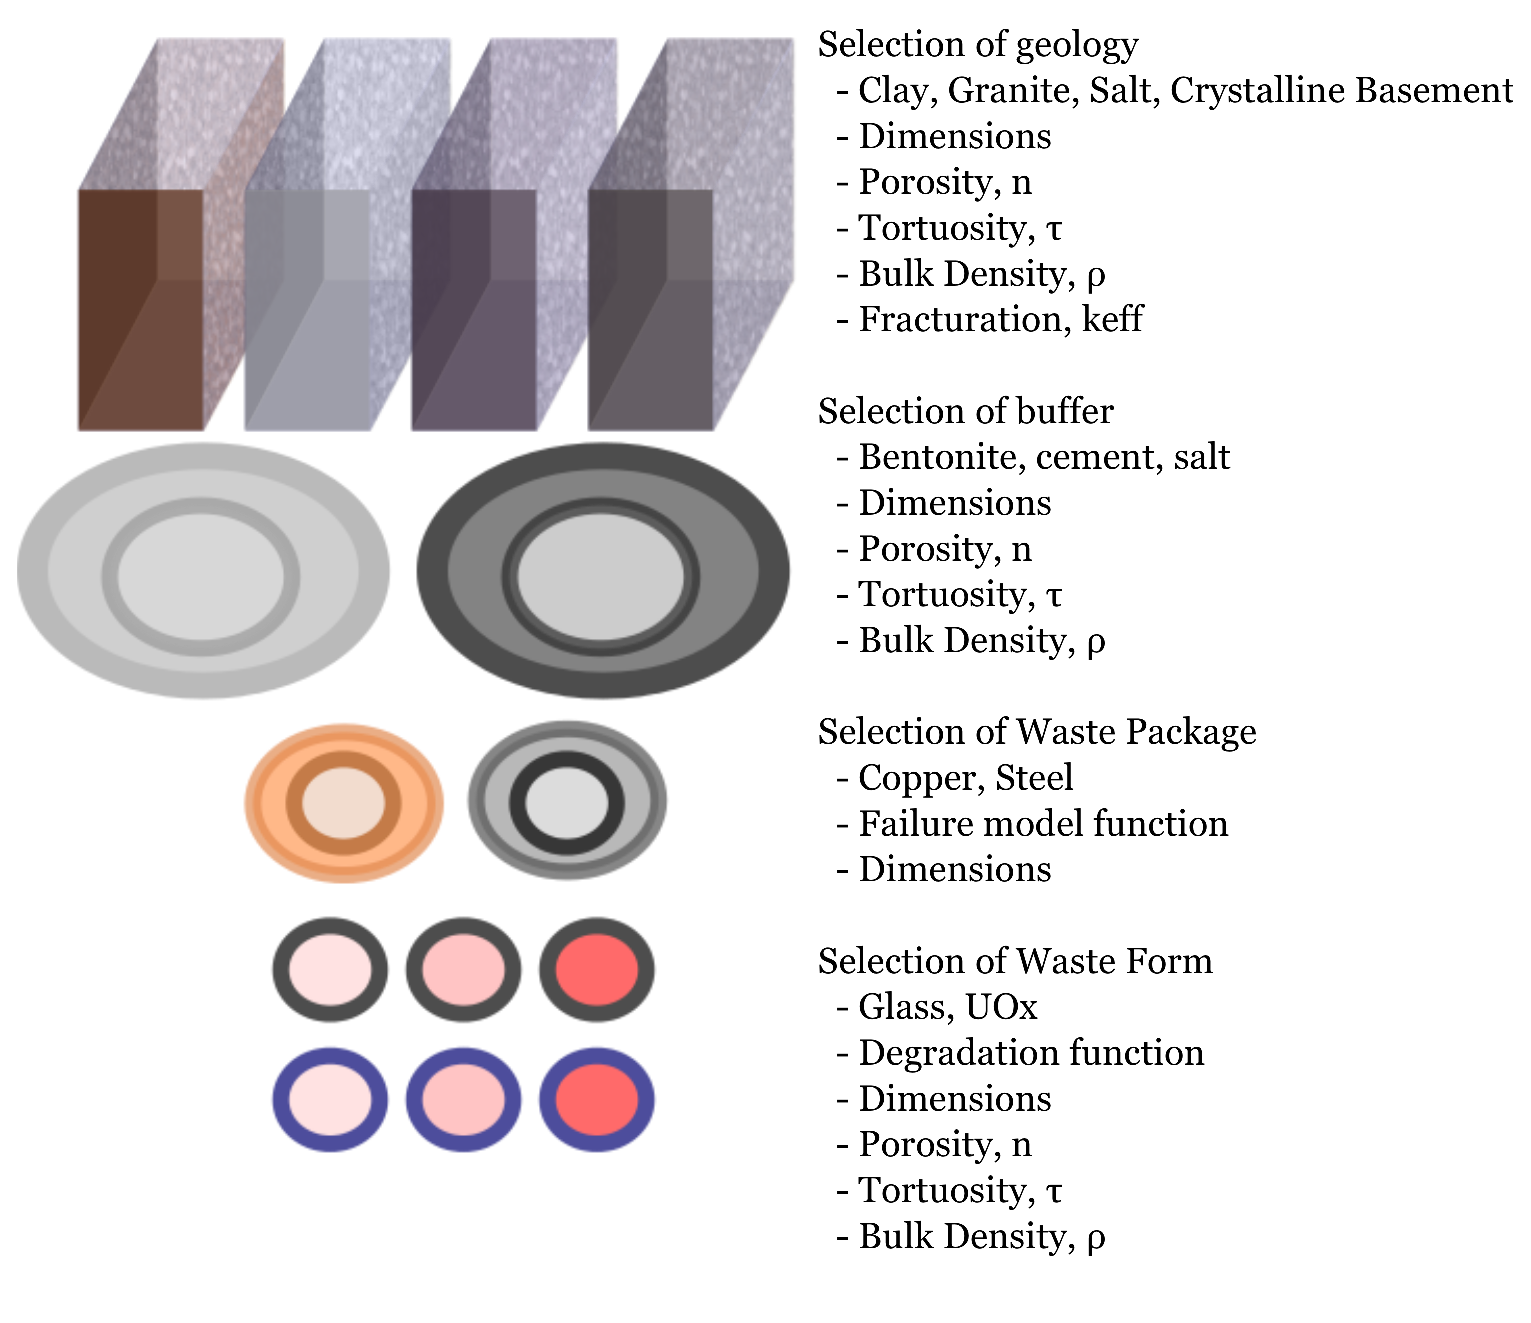
\includegraphics[height=0.8\textheight]{./images/components.eps}
  \end{figure}
\end{frame}

\begin{frame}[ctb!]
  \frametitle{Base Case : Waste Form Abstraction}
  \begin{minipage}{0.45\textwidth}
    \begin{figure}[h!]
      \begin{center}
        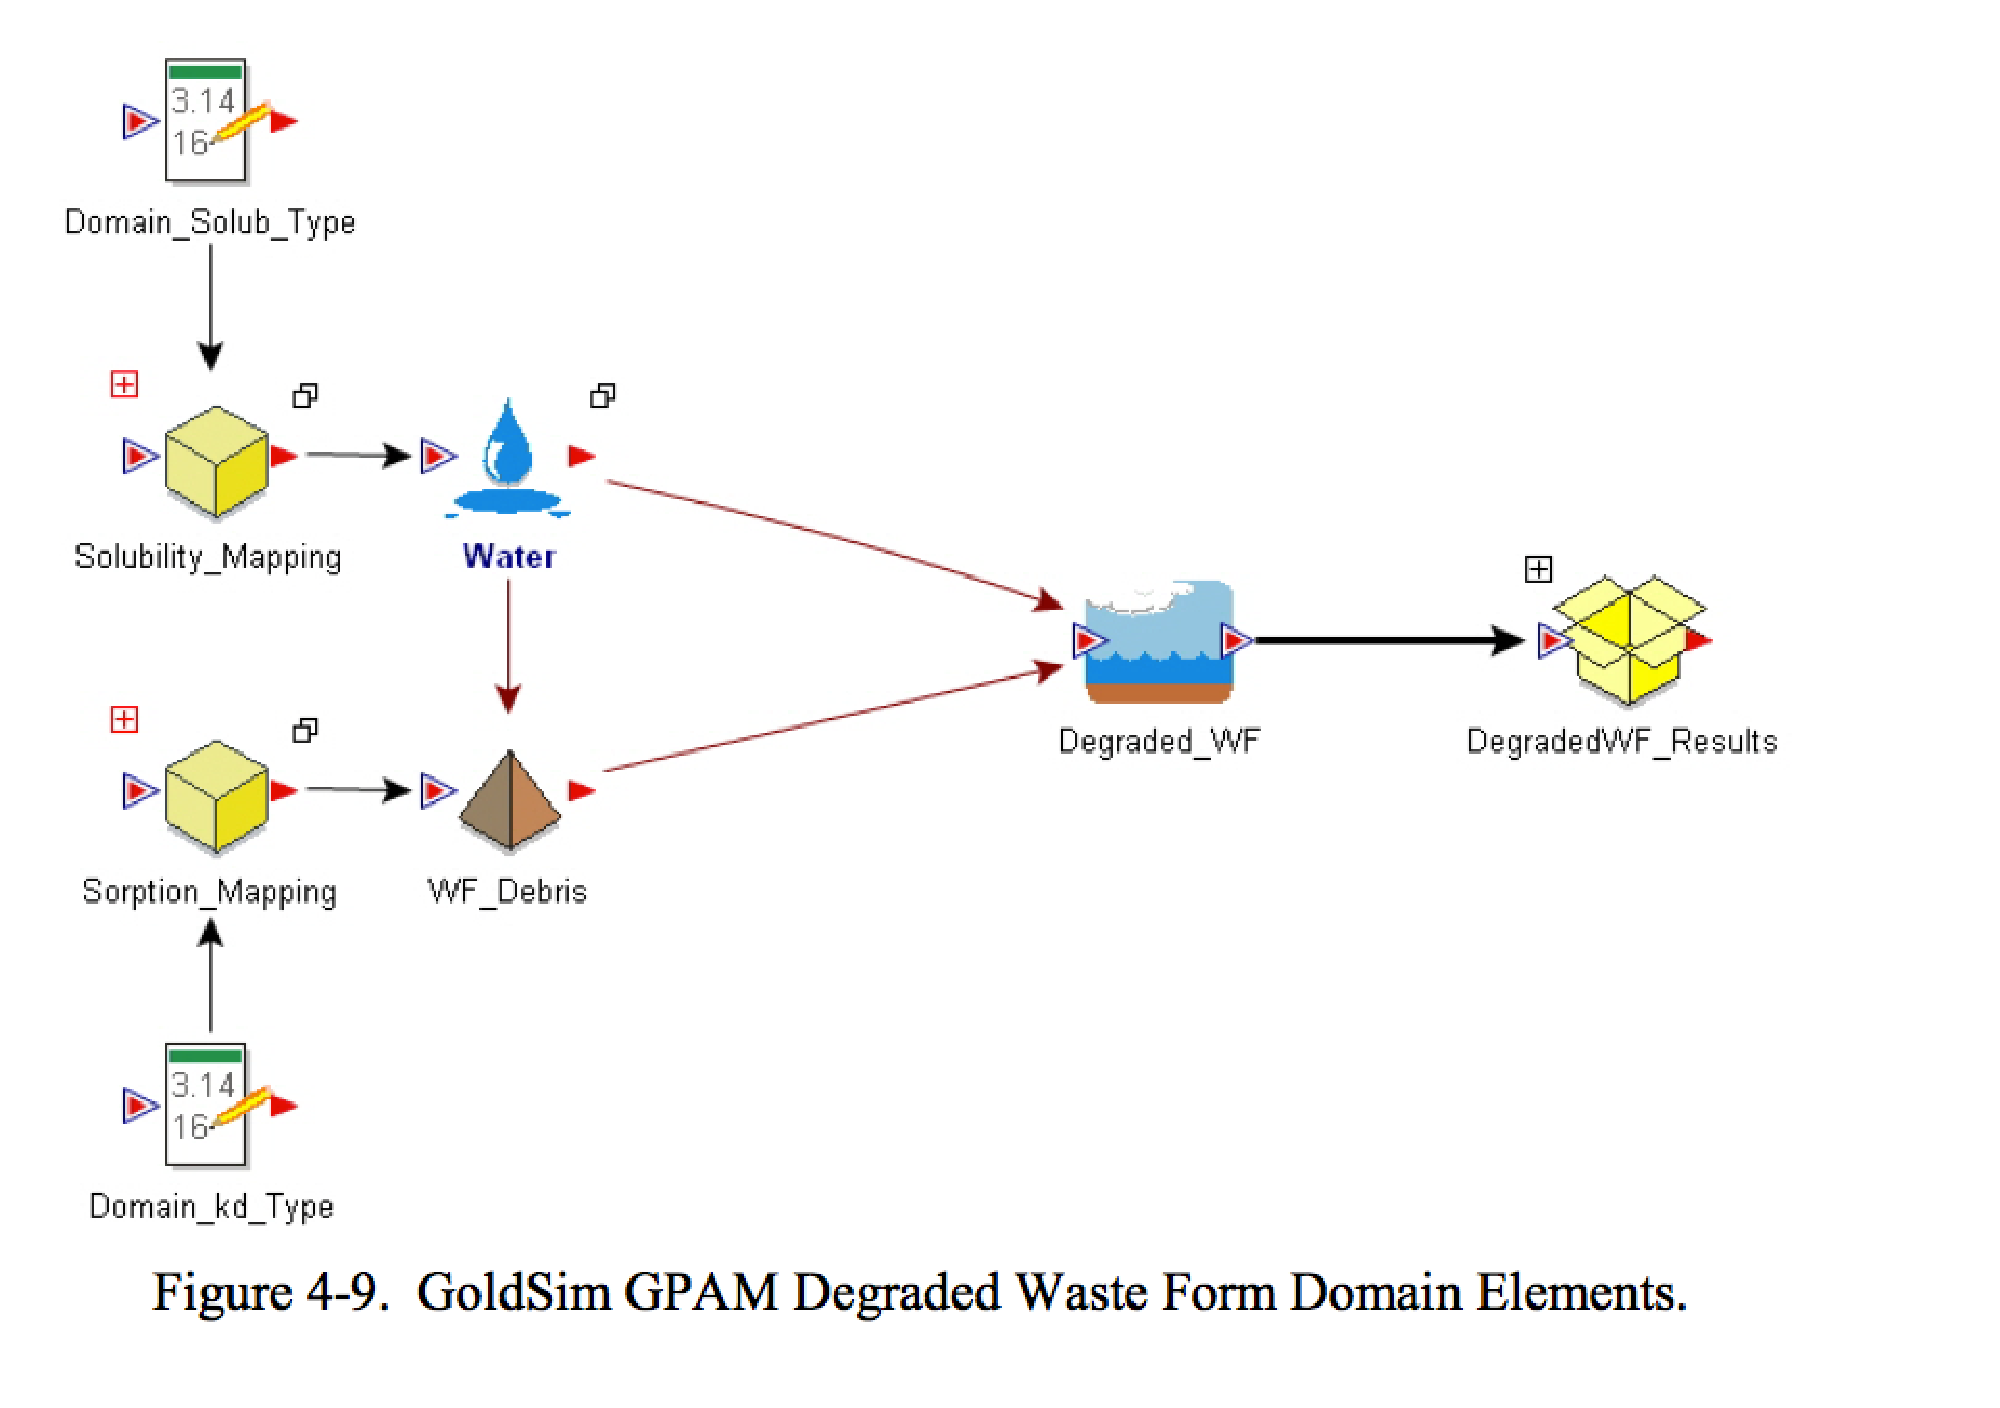
\includegraphics[width=\textwidth]{./images/wf.eps}
      \end{center}
    \end{figure}
  \end{minipage}
  \hspace{0.01cm}\large{$\rightarrow$}\hspace{0.01cm}
  \begin{minipage}{0.45\textwidth}
    \begin{figure}[h!]
      \begin{center}
        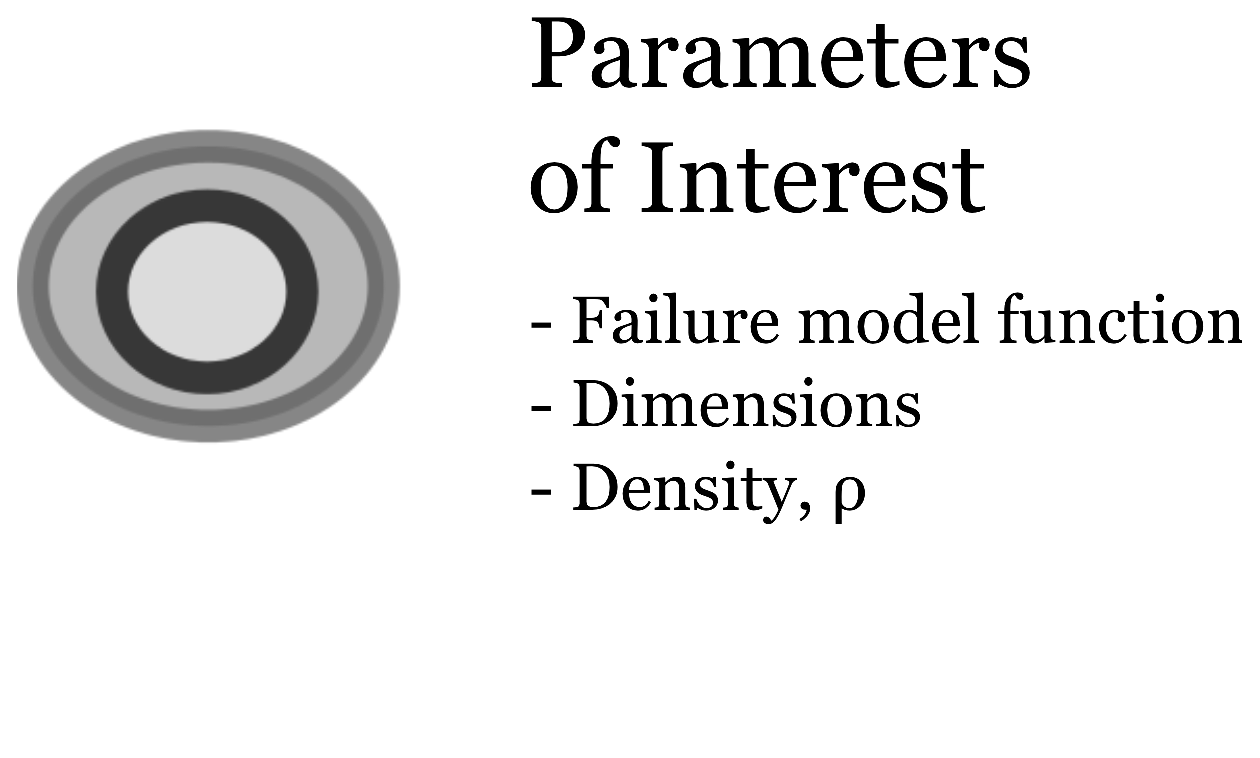
\includegraphics[width=\textwidth]{./images/abstractionWF.eps}
      \end{center}
    \end{figure}
  \end{minipage}
\end{frame}

\begin{frame}[ctb!]
  \frametitle{Base Case : Waste Package Abstraction}
  \begin{minipage}{0.45\textwidth}
    \begin{figure}[h!]
      \begin{center}
        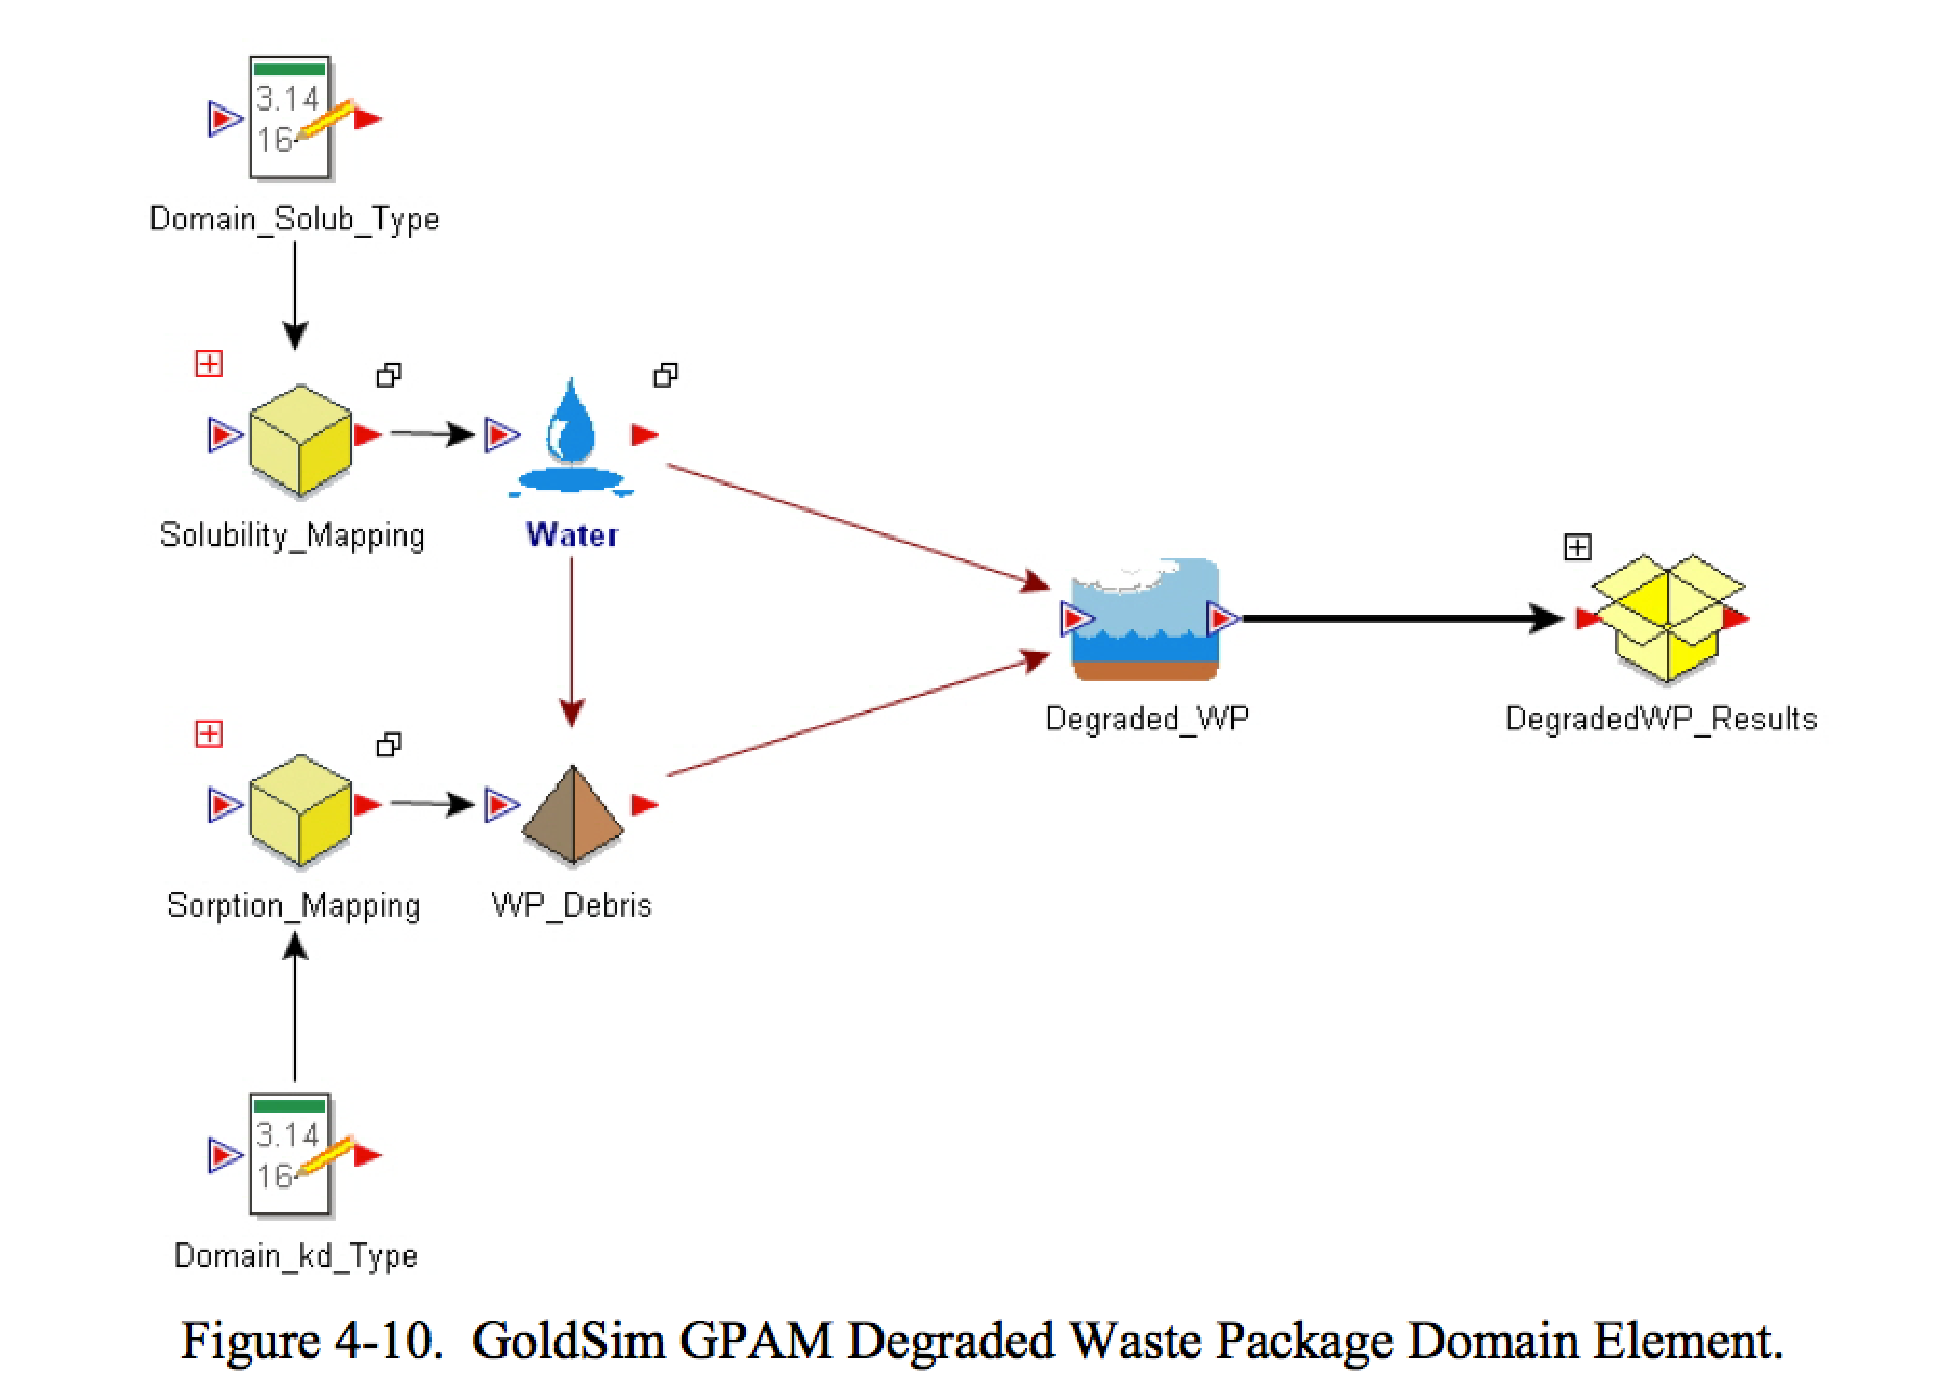
\includegraphics[width=\textwidth]{./images/wp.eps}
      \end{center}
    \end{figure}
  \end{minipage}
  \hspace{0.01cm}\large{$\rightarrow$}\hspace{0.01cm}
  \begin{minipage}{0.45\textwidth}
    \begin{figure}[h!]
      \begin{center}
        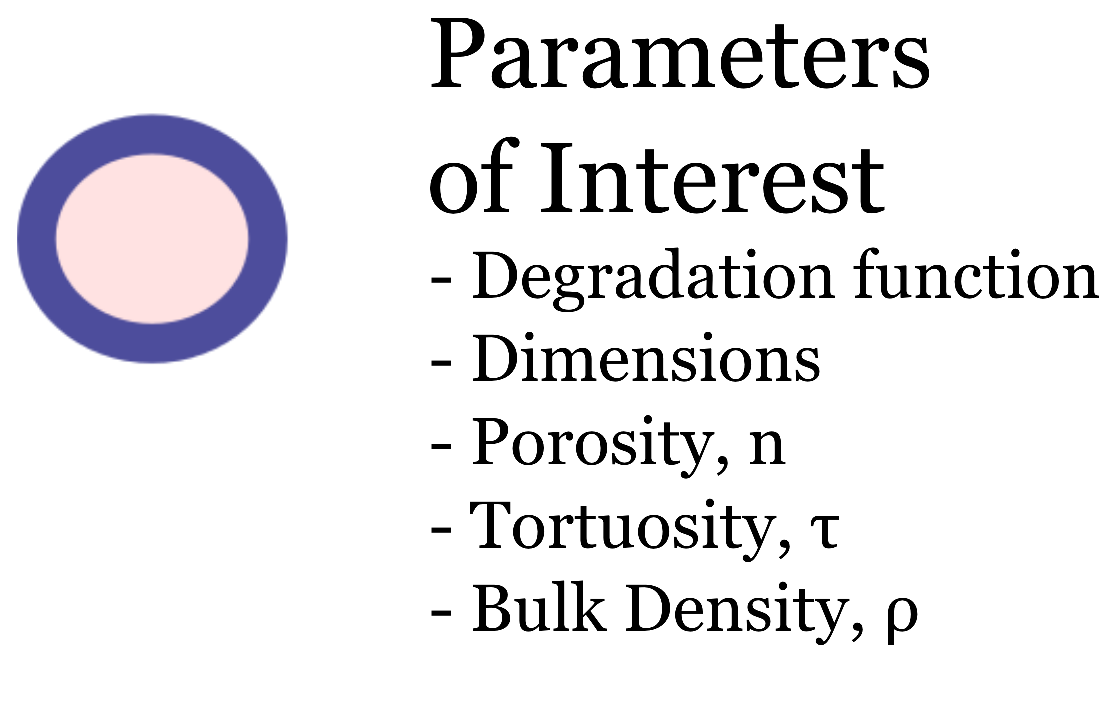
\includegraphics[width=\textwidth]{./images/abstractionWP.eps}
      \end{center}
    \end{figure}
  \end{minipage}
\end{frame}

\begin{frame}[ctb!]
  \frametitle{Base Case : Buffer Abstraction}
  \begin{minipage}{0.45\textwidth}
    \begin{figure}[h!]
      \begin{center}
        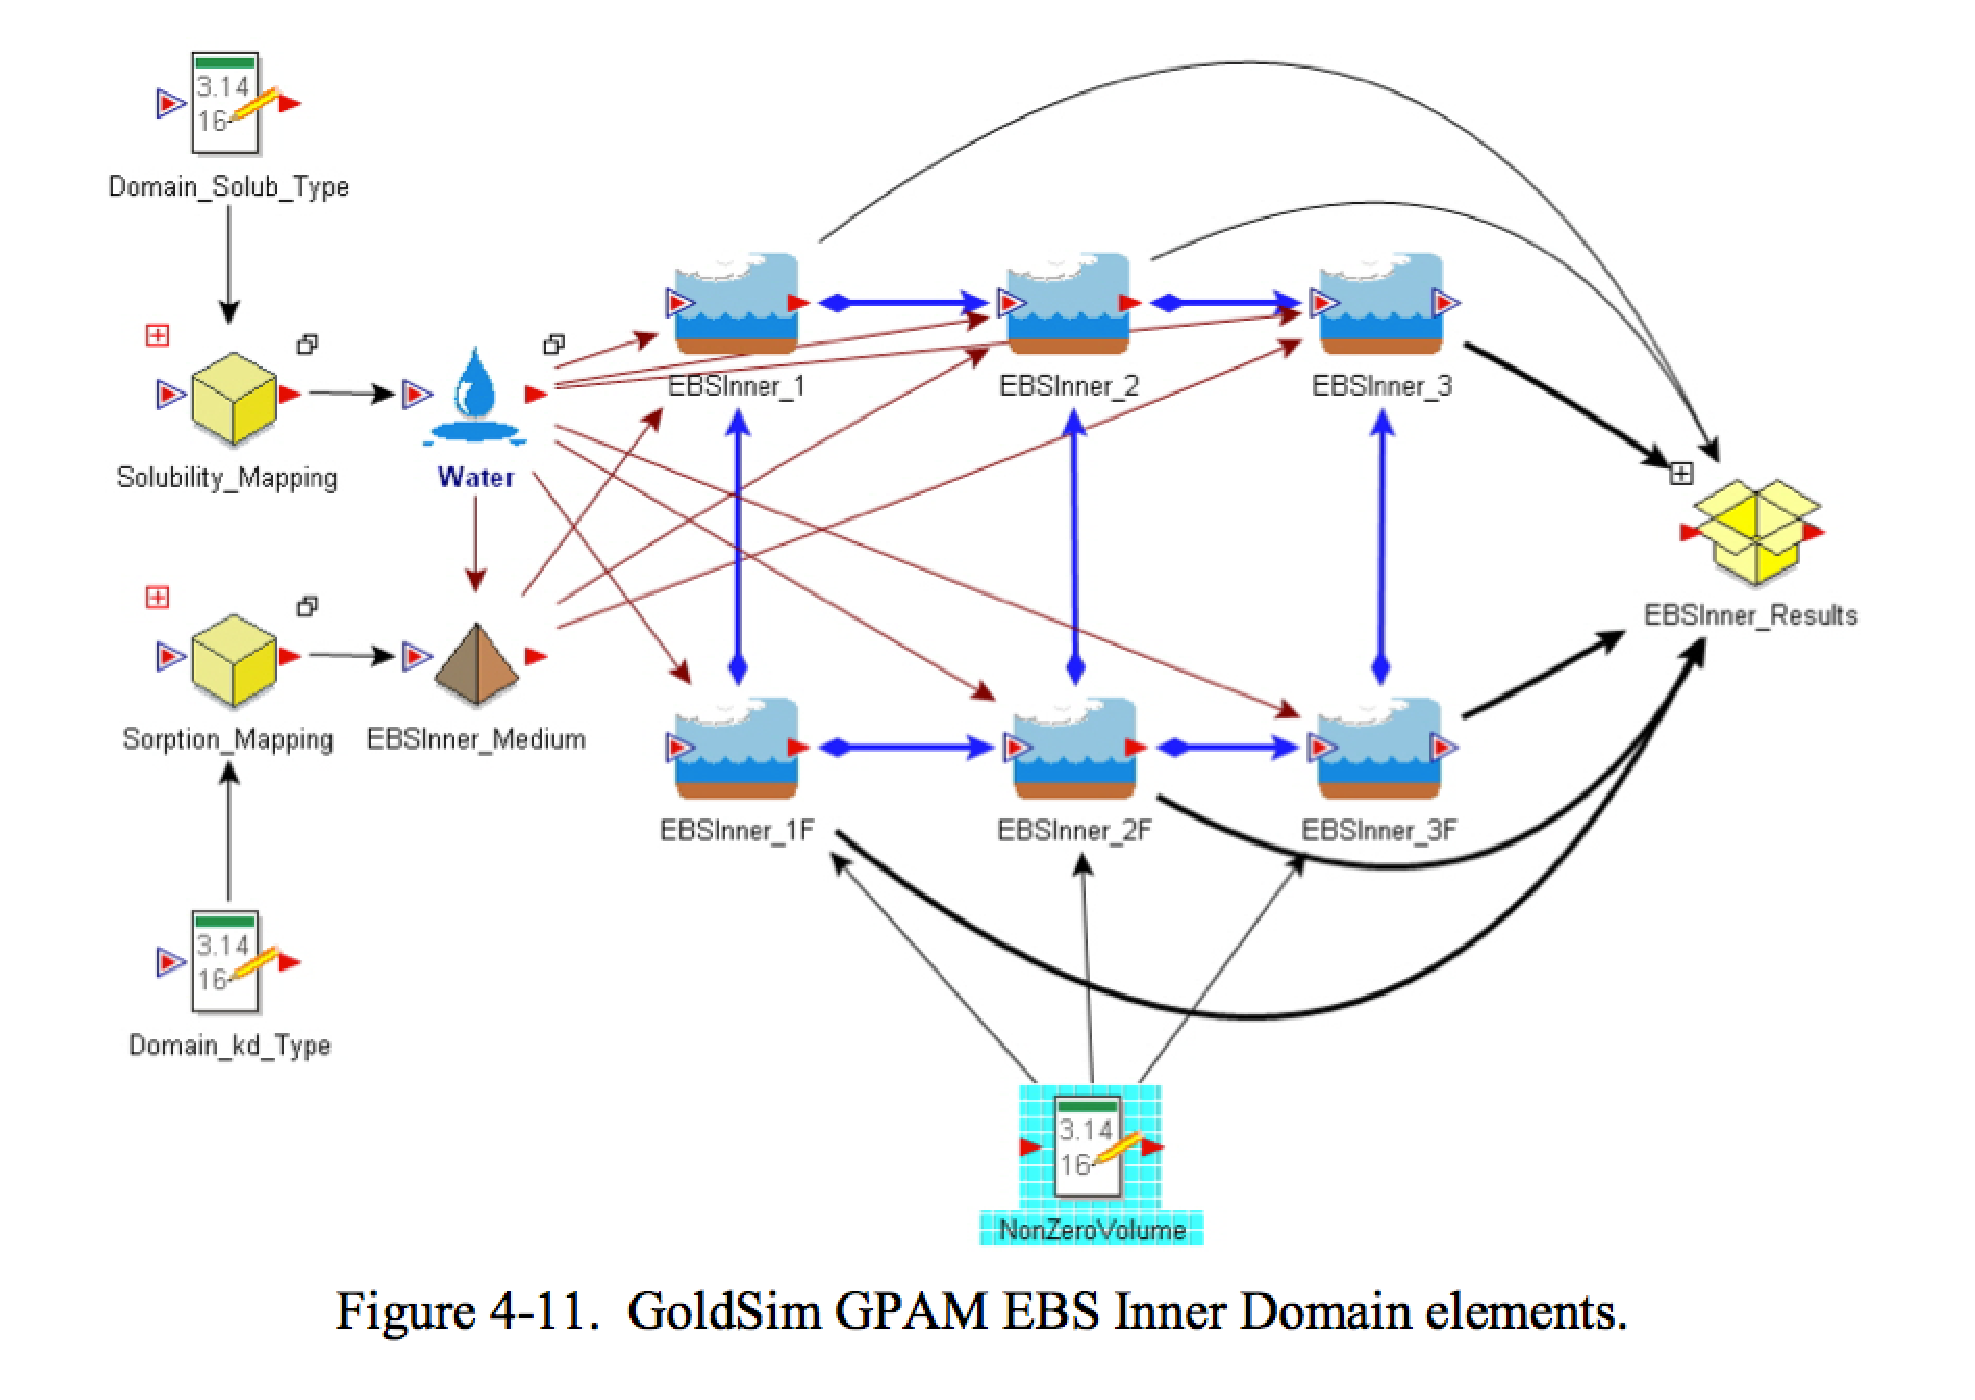
\includegraphics[width=\textwidth]{./images/buffer.eps}
      \end{center}
    \end{figure}
  \end{minipage}
  \hspace{0.01cm}\large{$\rightarrow$}\hspace{0.01cm}
  \begin{minipage}{0.45\textwidth}
    \begin{figure}[h!]
      \begin{center}
        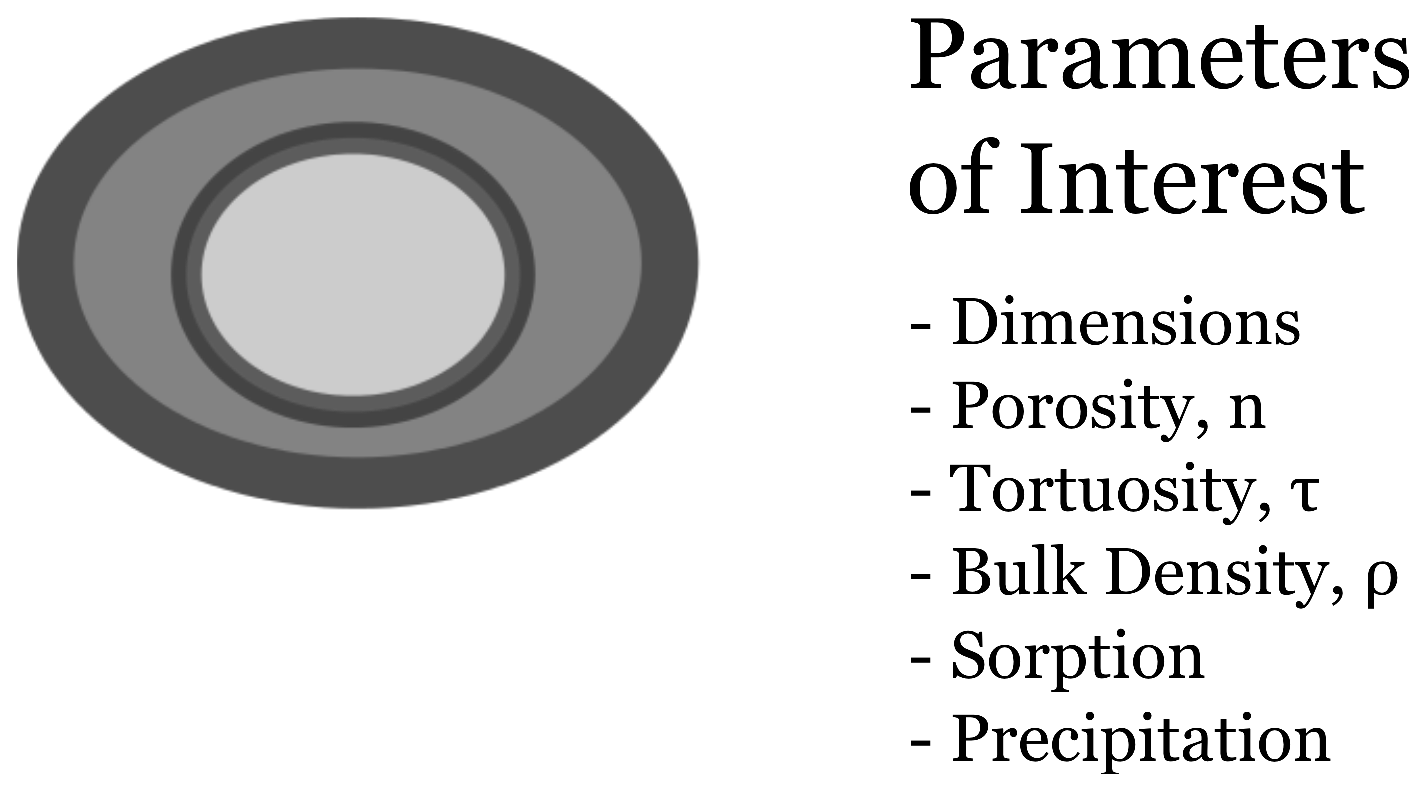
\includegraphics[width=\textwidth]{./images/abstractionBuffer.eps}
      \end{center}
    \end{figure}
  \end{minipage}
\end{frame}

\begin{frame}[ctb!]
  \frametitle{Base Case : Geology Abstraction}
  \begin{minipage}{0.45\textwidth}
    \begin{figure}[h!]
      \begin{center}
        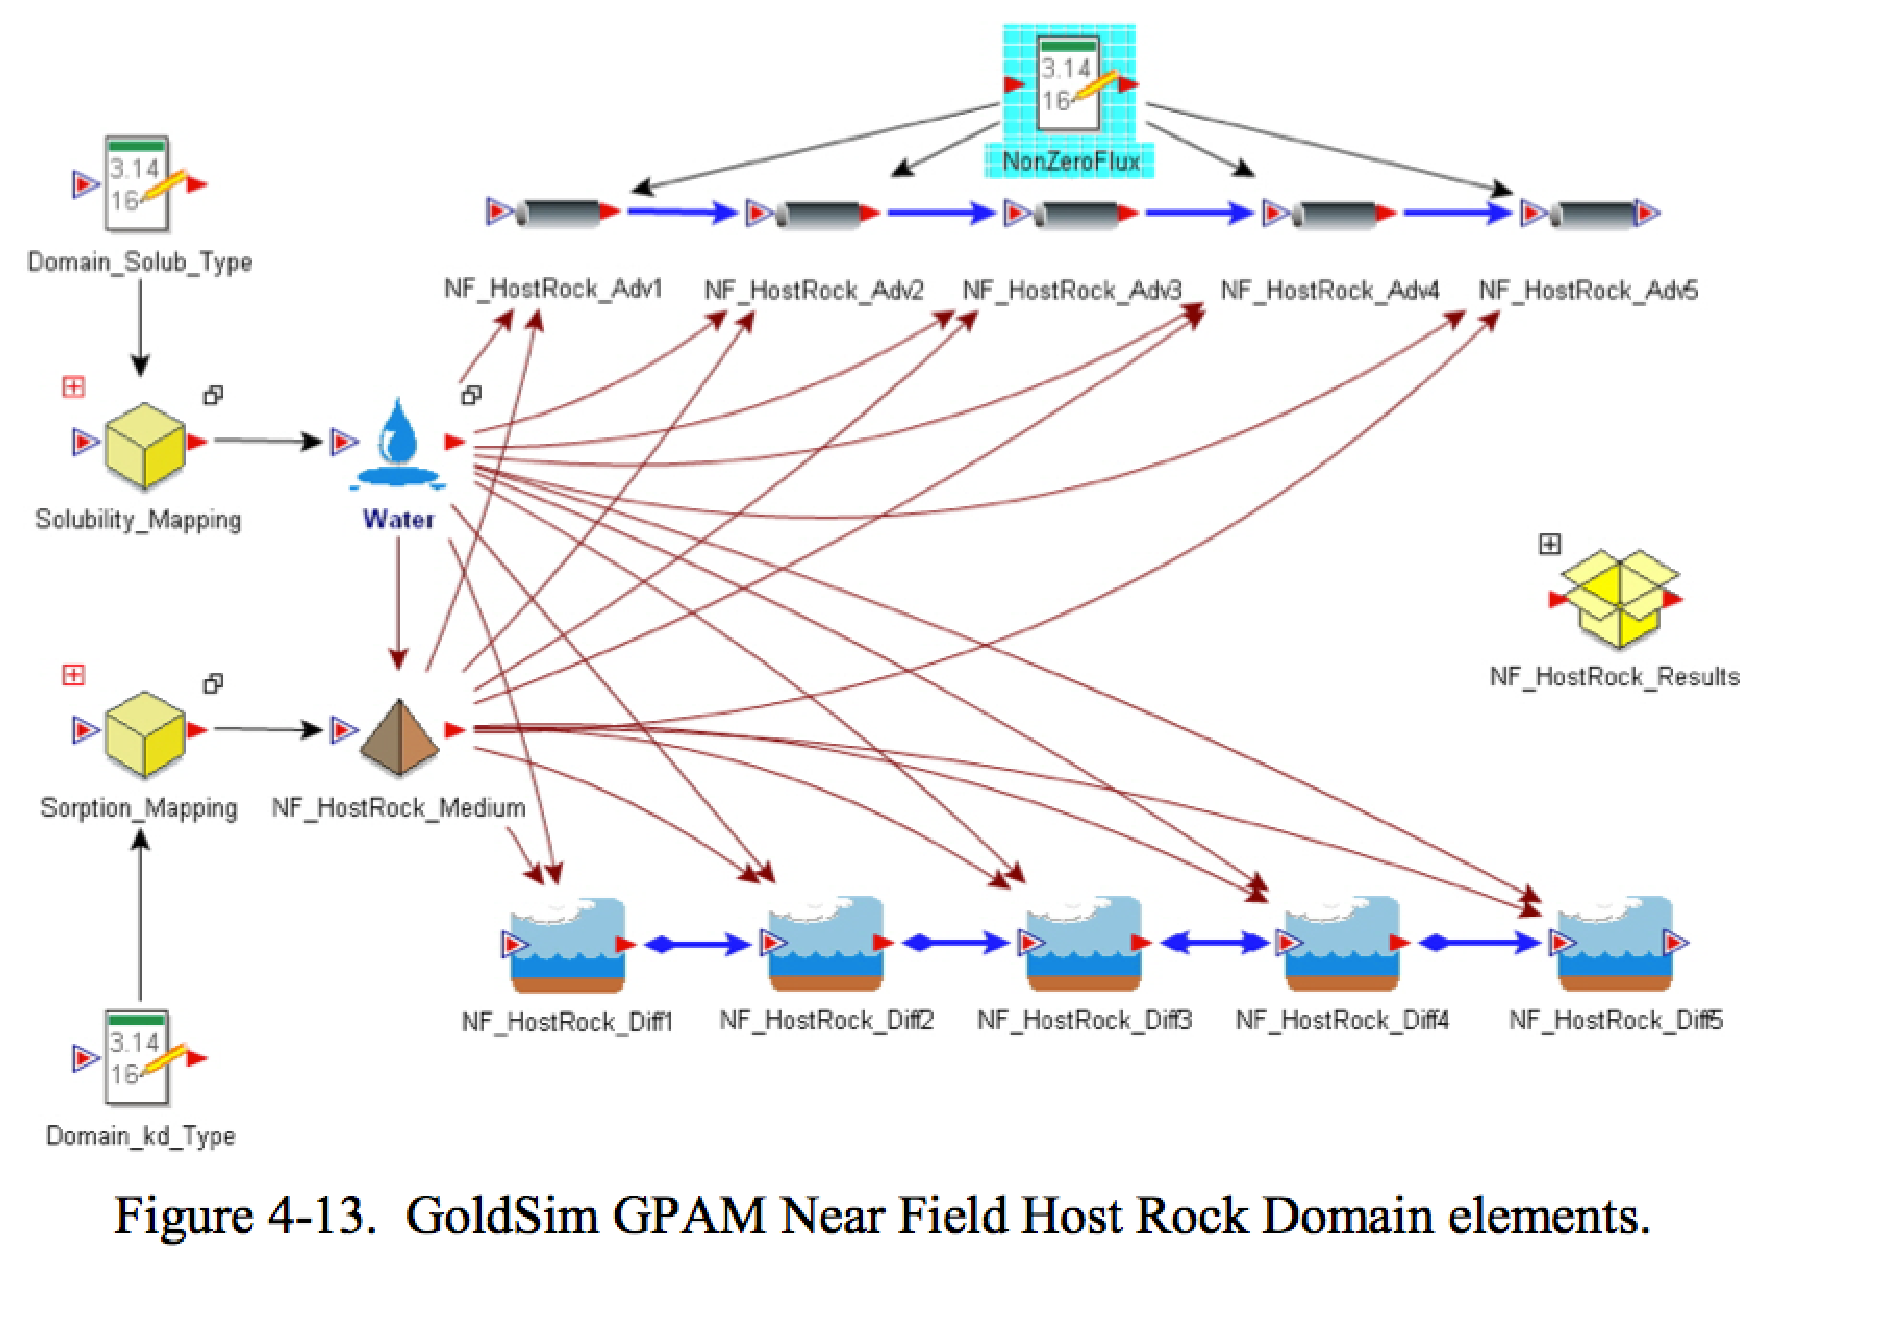
\includegraphics[width=\textwidth]{./images/rock.eps}
      \end{center}
    \end{figure}
  \end{minipage}
  \hspace{0.01cm}\large{$\rightarrow$}\hspace{0.01cm}
  \begin{minipage}{0.45\textwidth}
    \begin{figure}[h!]
      \begin{center}
        \includegraphics[width=\textwidth]{./images/abstractionRock.eps}
      \end{center}
    \end{figure}
  \end{minipage}
\end{frame}

\begin{frame}[ctb!]
  \frametitle{Base Case : System Level Abstraction}
  \begin{figure}[h!]
      \includegraphics[width=\textwidth]{./images/abstractionSystem.eps}
    \caption{System level abstraction seeks to determine the systems level 
    response to the change in models of subcomponents.}
  \end{figure}
\end{frame}
